\chapter{Model bursting behavior (oscillation) of neurons}

The very first non-Hodgkin-Huxley model that can produce oscillation is
Fitzhugh-Nagumo model (Sect.\ref{sec:fitzh-nagumo-model}).


\section{Hodgkin-Huxley model (1952)}

Hogdkin-Huxley model (Sect.\ref{sec:Hodgkin-Huxley-1952-model}) is the first to
provide a quantitative analysis of oscilation in membrane potential in the form
of APs (Sect.\ref{sec:AP-neuron}).

There are 4 ODEs in Hodgkin-Huxley model: membrane potential $V_m$, and three
gating variables $m, h, n$ modeling the ionic transportation across the
membrane. Except $V_m$ is modeled using Ohmic linear equation, the three gating
variables are modeled using first-order ODE.


\section{FitzHugh-Nagumo model (1955-1960): BVP or Bonhoeffer-van der Pol}
\label{sec:fitzh-nagumo-model}
\label{sec:BVP}
\label{sec:Bonhoeffer-van-der-Pol}


The initial goal was to model the synchronization of firing of two snail neurons
using a simple model. ~\citep{fitzhugh1960tph} created 2-variable reduced model
that can reproduce characteristic of AP (e.g.
the threshold, the plateau, the transient
increase...)\footnote{\url{http://www.scholarpedia.org/article/FitzHugh-Nagumo_model}}.

\begin{equation}
\begin{split}
\dot{x} &= a \times \left( y  - f(x) + I_\app(t) \right) \\
\dot{y} &= b \times \left( g(x) - y \right)
\end{split}
\end{equation}
with $x$ represents the membrane potential, and $y$ is an internal, or recovery,
variable. 
\begin{itemize}
  \item $f(\cdot)$ is a cubic function
  \item $g(\cdot)$ is a linear function
  \item $a,b$ are time constants
  \item $I_\app(t)$ is the external, applied current. 
\end{itemize}
However, the oscillations do not fit accurately to many physical oscillators,
such as rapid firing of the neuron compared to the relative long interval
between spikes.

\subsection{-- Fitzhugh's work}

Based on the van der Pol system \citep{vanderPol1926}, a system of two
differential equations that possess non-linear relaxation oscillation
(Sect.\ref{sec:simplest-nonlinear-oscill}), two years later,
\citep{fitzhugh1961ips} extended the model, created a model called {\bf
Bonhoeffer-van der Pol model} (BVP for short), that can reproduce osccillations
(the formation of trains of impulse), e.g. tonic spiking in neurve cells, and
then apply to $(V_m,n)$ fast-slow reduced model.

The equation extended from eq.\eqref{eq:vanderPol-Lienard} by adding new terms
[NOTE: $a=b=I_\app=0$ the equations is the original van der Pol equation]
\begin{eqnarray}
    \dot{x} &&= \varepsilon \left( x-\frac{1}{3}x^3 - y + I_\app \right) \\
    \dot{y} &&= \frac{1}{\varepsilon}(x -a + by)
\end{eqnarray}
with $1-2b/3 <a < 1; 0 < b< 1; b< \varepsilon^2$. The condition guarantees that
when $I_\app=0$, there is only one singular point
(Sect.\ref{sec:singular-points}), which is a stable node or focus, representing
the {\it resting state}.  

Here, we use $\varepsilon$ instead of $\mu$, to indicated that
$\varepsilon\ll1$.
This is the famous dimensionless two-variable form of the model in polynomial
form, known as {\bf FitzHugh-Nagumo model of excitability}.  There are many
equivalent forms \citep{rocsoreanu2000}. A more general form is
\begin{eqnarray}
\varepsilon\dot{x} &&= f(x,y) + I_\app \\
\dot{y} &&= g(x,y)
\end{eqnarray}
with $g(x,y)$ is the y-nullcline, $f(x,y)$ is the x-nullcline (with cubic
shape). There is only one intersection of the two nullclines. 


\subsection{-- Nagumo's work}
%\subsection{Mathematical model}
\label{sec:mathematical-model-4}


To study the importance of stability in Hodgkin-Huxley system, 4 ODEs is
hard to analyze.


\citep{nagumo1962} represented FitzHugh model by an electrical device: the fast
variable is a non-linear current-voltage device, the recovery variable is the
resistor, inductor, and battery in series, as well as the membrane capacitor;
and proposed a modification of the non-linear diffusion equation that allow the
AP to return to the resting level (detail: read \citep{keener2008}). Thus, the
model is often known as Fitzhugh-Nagumo model.

\citep{nagumo1962} then developed the spatially distributed FitzHugh-Nagumo
model where diffusion is added to the general FitzHugh-Nagumo model
\begin{eqnarray}
\varepsilon \frac{\partial v}{\partial t}  &&= \varepsilon^2 \frac{\partial^2
v}{\partial x^2} + f(v,w) + I_\app \\
\frac{\partial w}{\partial t} &&= g(v,w)
\end{eqnarray}
This model has different travelling waves depending on the choices of parameters
of the system.

In this system, $y$ is the more slowly changes than $x$, except near the
$y-$nullcline, Fig.\ref{fig:FitzHugh_nullclines}. The $x$-nullclines has
N-shaped cubic; the three parts are called left, middle, and right branches. The
figure showes P=resting point. The location of this point, and its stability
depends on $I_\app$. The condition being used above guarantees P is stable when
$I_\app=0$. Fig.\ref{fig:FitzHugh-singularpoint} shows a different
location of the singular point when a stimulus is applied $I_\app=-0.128$; while
a positive stimulus current move the x-nullclines downward, e.g. $I_\app=0.4$. 

\begin{figure}[hbt]
  \centerline{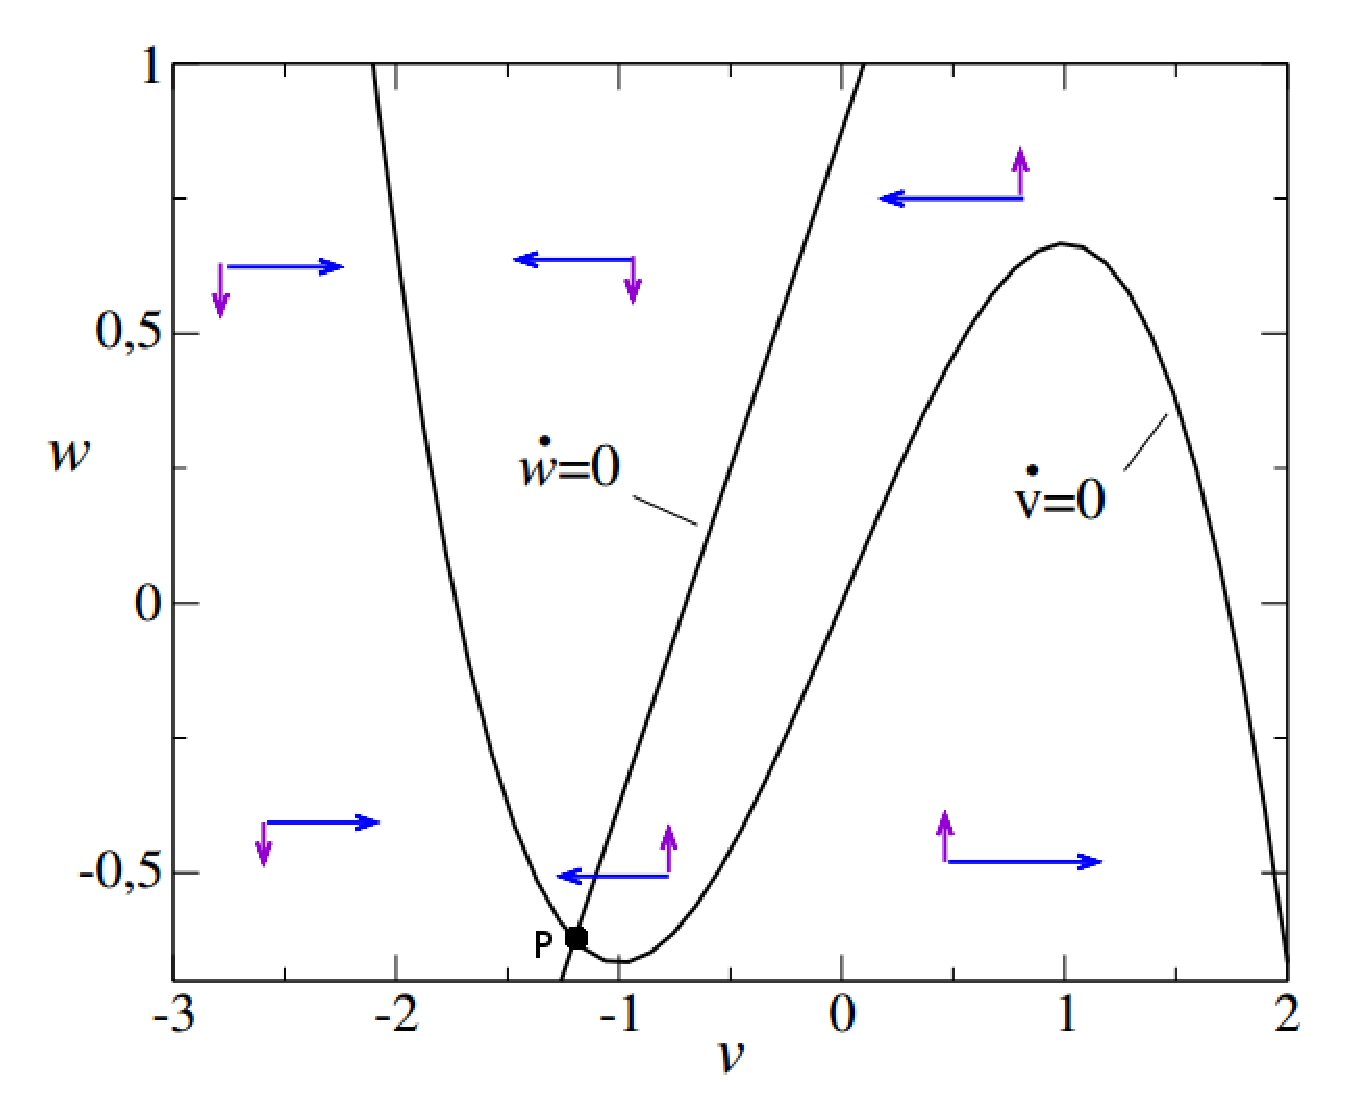
\includegraphics[height=4.5cm,
    angle=0]{./images/FitzHugh_nullclines.eps}
    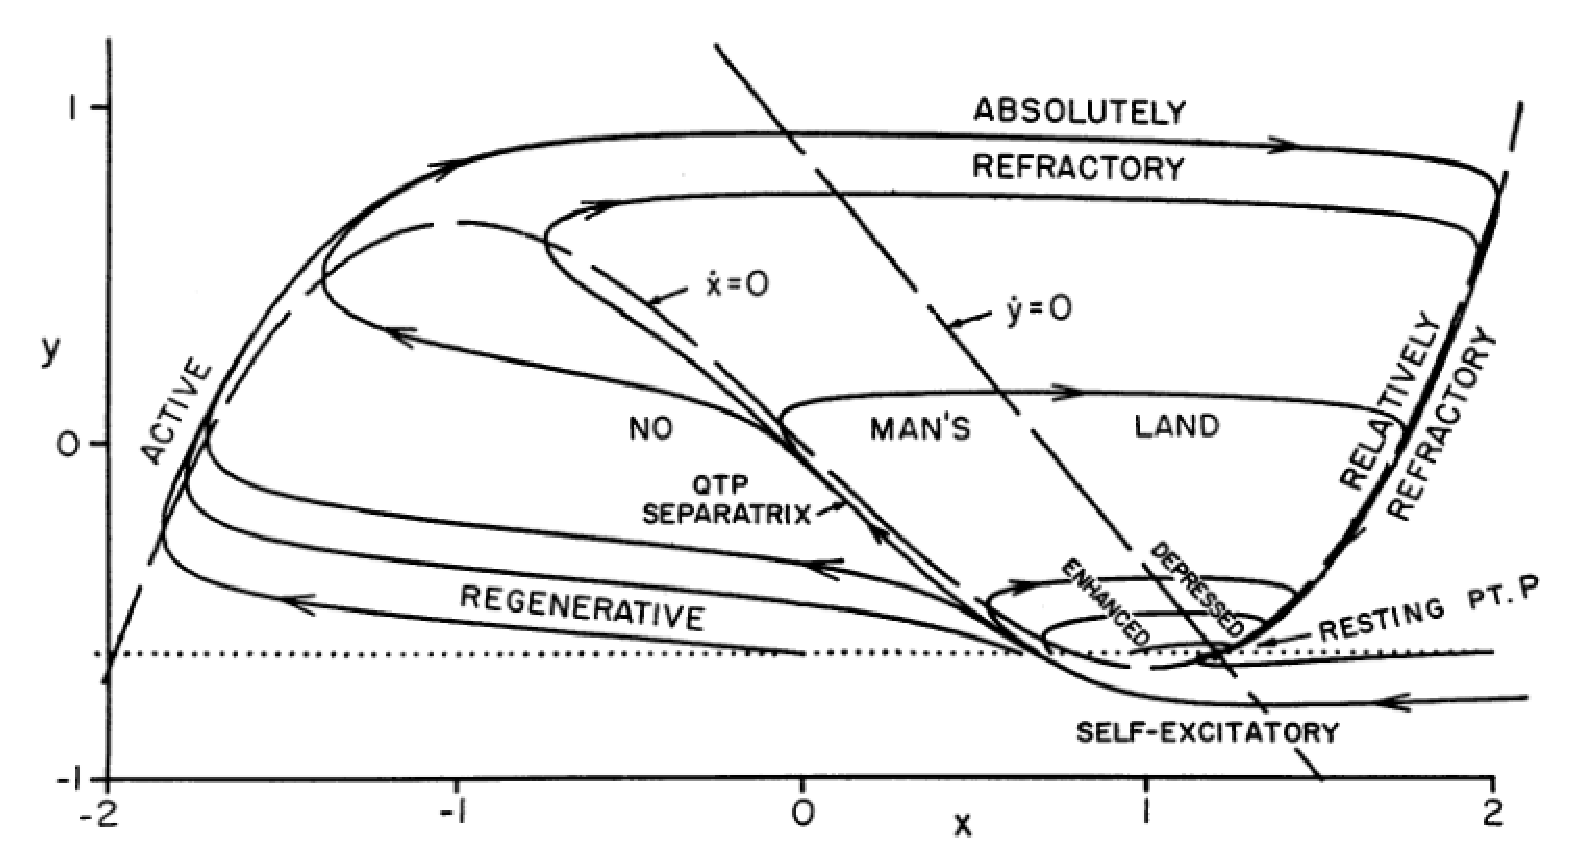
\includegraphics[height=4.5cm,
    angle=0]{./images/FitzHugh_nullclines-original.eps}
    }
  \caption{The nullclines using the current equations (left); and the one in the
  original paper (right), both with $I_\app=0$. The difference is that $y$ here
  (slope 1/b) is indeed $-y$ in the original paper (which has slope -1/b). Dotted line = locus of
  initial condition}
  \label{fig:FitzHugh_nullclines}
\end{figure}

\begin{figure}[hbt]
  \centerline{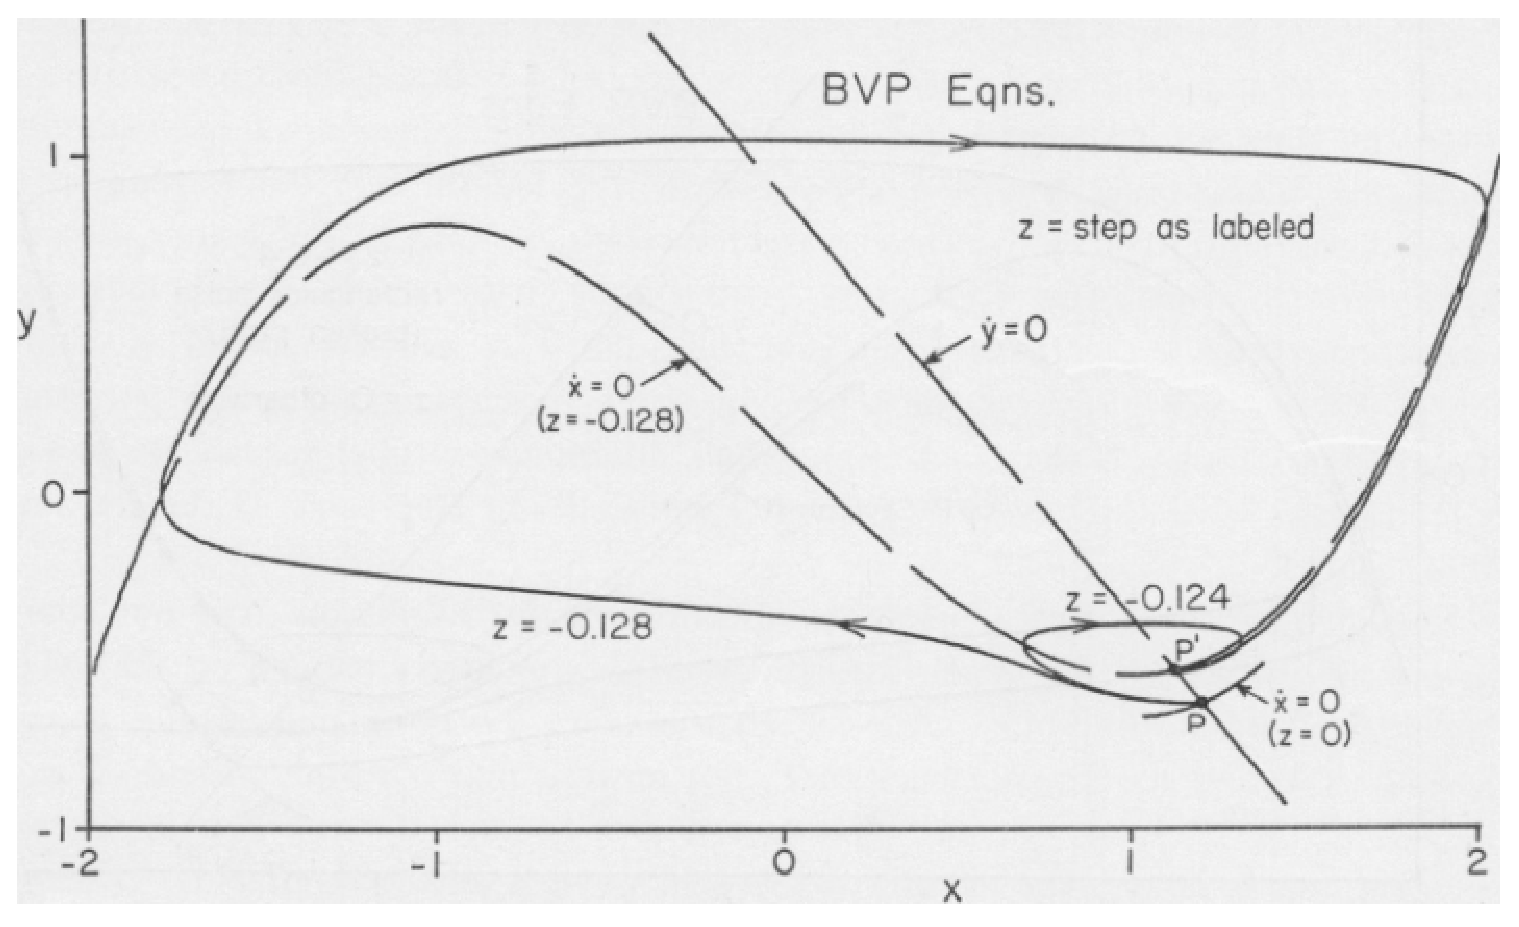
\includegraphics[height=5cm,
    angle=0]{./images/FitzHugh_nullclines-original_2.eps}}
  \caption{The nullclines with $I_\app=z=-0.128$. Here, P' is the new stable
  singular point (P is the point when $I_\app=0$)}
  \label{fig:FitzHugh-singularpoint}
\end{figure}

% The BVP model has its counterpart in the Hodgkin-Huxley model. 
\begin{mdframed}
  Fitzhugh-Nagumo model is basically a quantitive analysis of the HH
  model. There is no new components added to the model.
\end{mdframed}
% {\bf Formulation}: It
% is reasonable to assume that ``m'' quickly reach its steady-state
% $m_\infty(V)$ under the stimulus, and the system is examined from that
% point.  So, it is assumed that $m$ reach the steady state when
% $t<0$. Another important notice is that the sum of
% $n_\infty(v)+h_\infty(v)=0.85$. This discovery was made by FitzHugh,
% as shown in Fig.~\ref{fig:HH_result}, and will be a factor to reduced
% the complexity of the model to 2D.


% Then, he introduced either $h$ or $n$ to the reduced system,
% making it a 3-parameter system. Finally, he investigate the complete
% system $V,m,n,h$. Thus, it provided an insight how the system change
% when considering individual parameters.
% % It means that $m$ quickly reach its steady state than $n$ and $h$.



\begin{figure}[hbt]
  \centerline{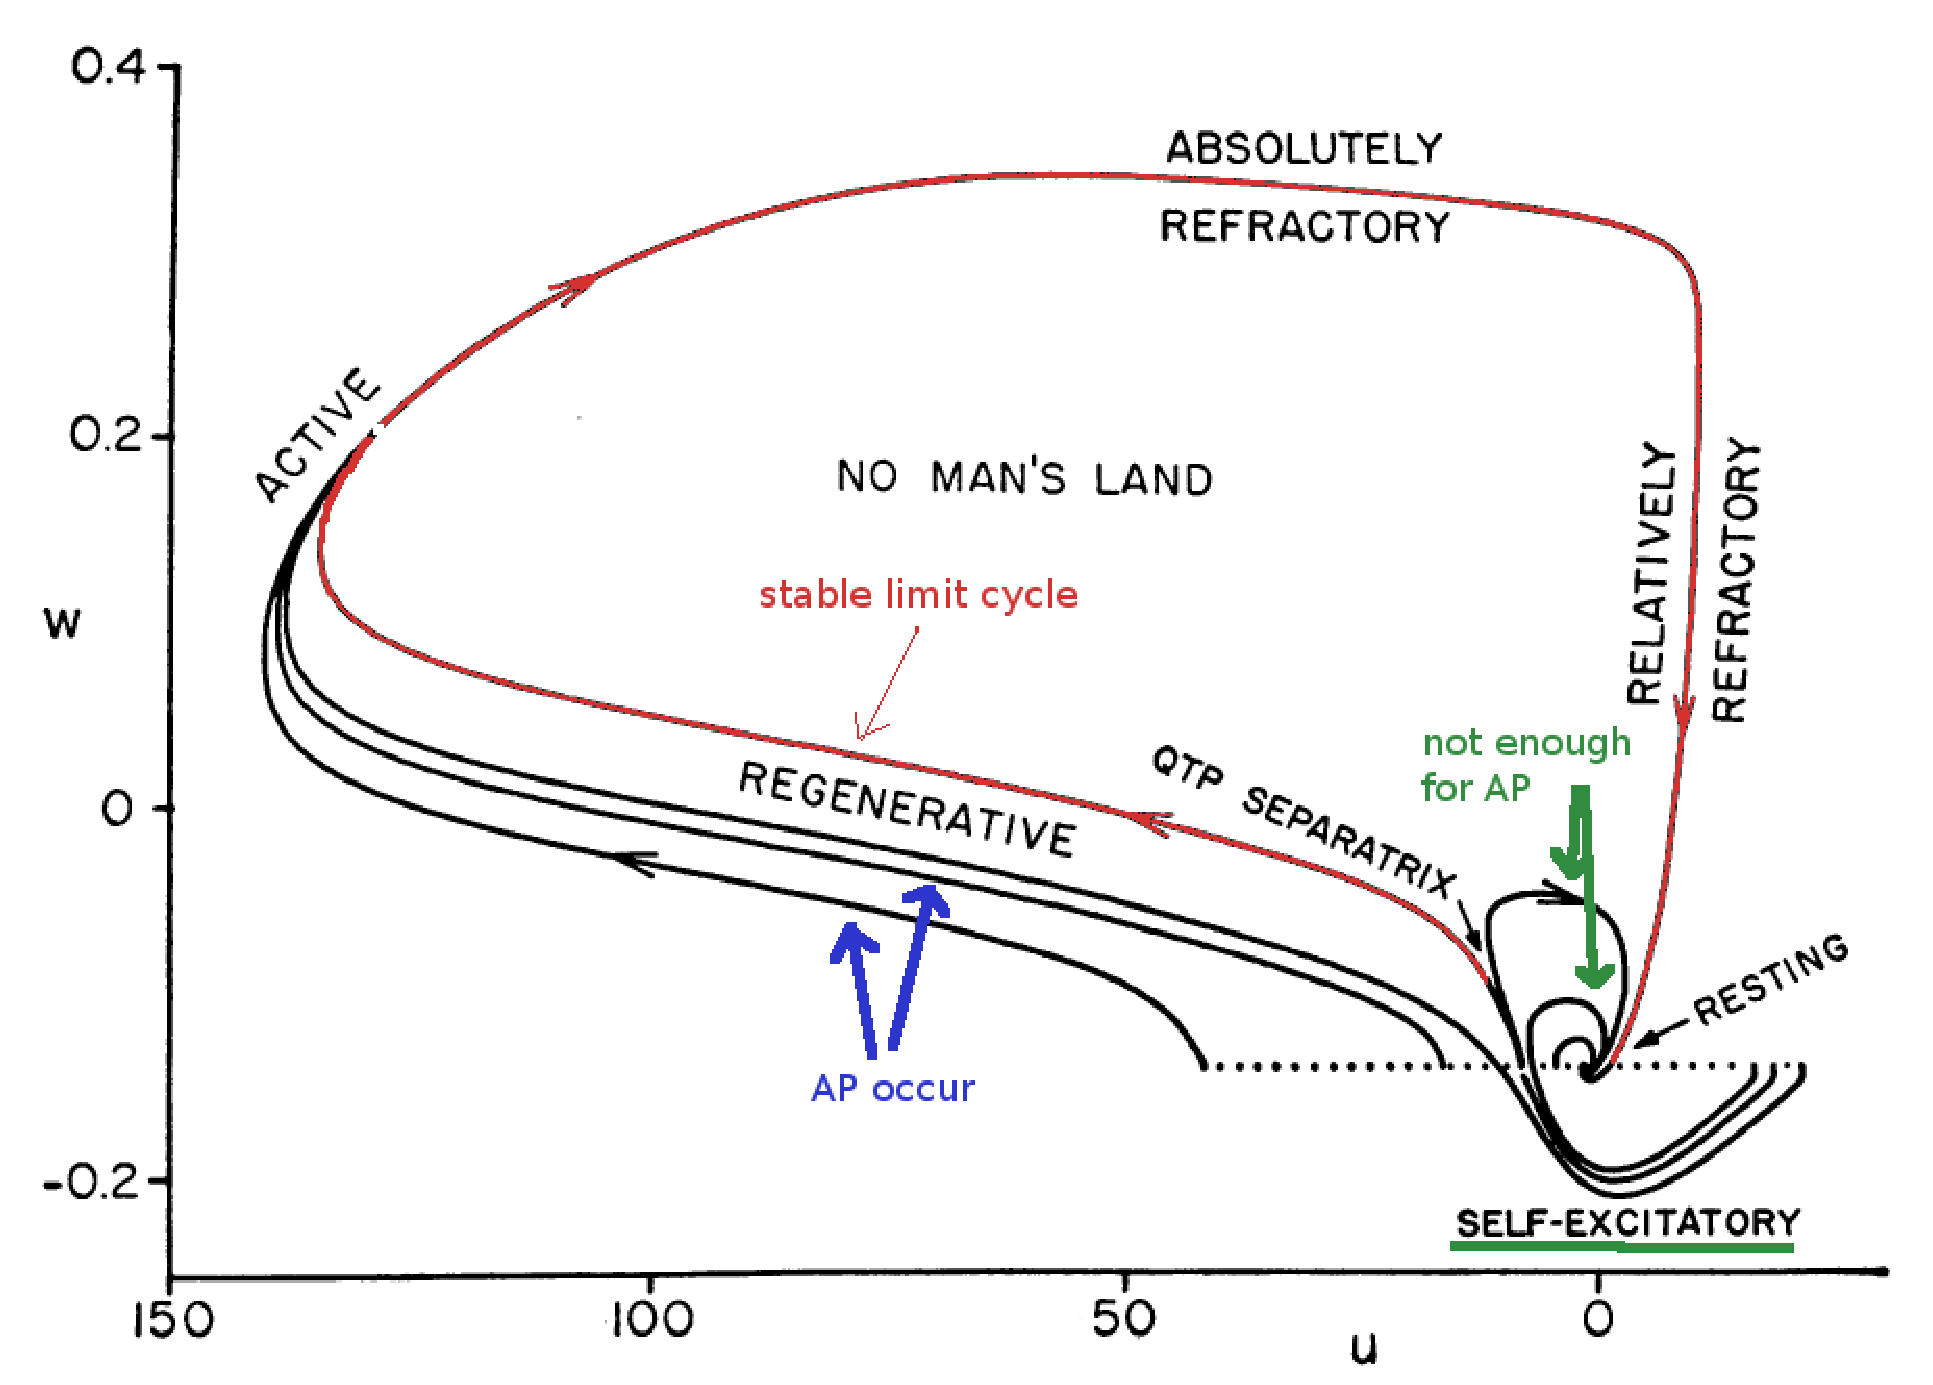
\includegraphics[height=5cm,
    angle=0]{./images/HH_phaseplane.eps}}
  \caption{HH projected onto (u,w) plane with $u=V_m+36m, w=(n-h)/2$
    ~\citep{fitzhugh1961ips}. NOTE: the sign of $V$ follow the new
    concept while the sign of $V_m$ in the paper follow
    Hodgkine-Huxley concept}
\label{fig:HH_phasespace}
\end{figure}

If we define $u=V_m+36m$, $w=0.5(n-h)$, then the path on $(w,u)$ is shown
in Fig.~\ref{fig:HH_phasespace}. Even though this is not the phase plane, since
each point in $(w,u)$ is just a projection of a plane of 4 dimensions
$(V,m,n,h)$, we can see three singular points: the {\it stable resting point},
{\it threshold saddle point} (i.e. any trajectory below this return to the
resting state, above this reach the excited point before returning to the
resting via refractory process), and {\it stable excited point}.



\subsection{Hypothesis analysis}

As described in Hodgkin-Huxley model (Sect.\ref{sec:Hodgkin-Huxley-1952-model}),
ionic currents through plasma membrane formed by the cation movements via ion
channels (potassium, sodium channels) and a small anion current through leak
channels are mathematically represented by the following equation.

\begin{equation}
  \label{eq:286}
     \Csc dv/dt = - \overline{g_{\ce{K}}}n^4(v-v_{\ce{K}}) - \overline{g_{\ce{Na}}}
    m^3h(v-v_{\ce{Na}}) - \overline{g_{\leak}} (v-v_{leak}) + I_\app
\end{equation}
with $v=V_m-V_r, v_i=E_i-V_r$, $V_m$ is the membrane potential, $E_i$
is the reversal potential of the corresponding ion channels following
Nernst equation, $V_r$ is the membrane resting potential.

HH model has 4 ODEs with 4 variables of state
($v,m,n,h$) in which $n, m, h$ are hypothesized
{\it membrane potential-dependent gating variables} whose dynamics are
assumed to follow {\it first-order kinetics}.
\begin{equation}
  \label{eq:285}
  \frac{dw}{dt} = -\frac{w-w_\infty}{\tau_w}, \; \text{ with }w=n, m, h
\end{equation}
where $\tau_w$ is time constants and $w_\infty$ is the fraction of gating
channels at the inner side of the membrane at equilibrium. The time constant of
$v$ is C$/g_m$ with C is the membrane capacitance, and $g_m$ is total membrane
conductance. 


\begin{figure}[hbt]
  \centerline{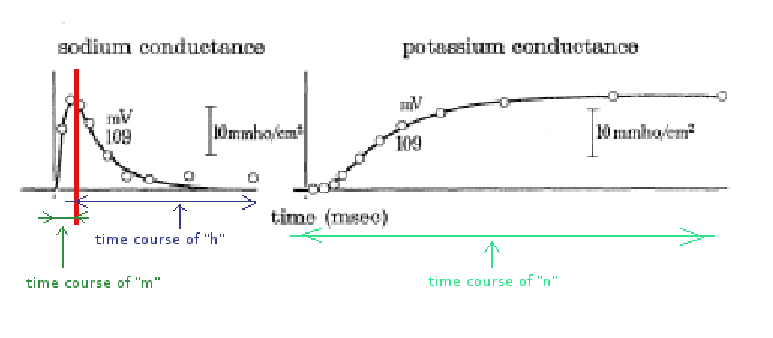
\includegraphics[height=4.5cm,
    angle=0]{./images/time_course.eps}}
  \caption{Time course of ``m'', ``n'', and ``h''}
  \label{fig:time_course}
\end{figure}


\subsection{Fast phase-plane analysis}
\label{sec:quant-analys}

To study the behavior of a dynamical system (typically a set of ODEs),
mathematicians developed a techniqued called {\it phase plane analysis}
(with nullcline plots) whose essential concept can be referenced in
Appendix.~\ref{chap:phase-plane-analysis}.
There are tools to automate this task and visualize instantly; users just need
to click on the plane to give the initial condition, it will generate the
trajectory automatically, i.e. how the system goes for a given initial input. 

Phase plane analysis works nicely for a system with 2 dependent variables as it
can be easily plot on a 2D plane. To reduce the number of dimensions in the
Hodgkin-Huxley model, currently with 4 degree of freedoms, Fitzhugh observed
that: $n$ and $h$ have slow kinetics relative to $V$ and $m$, i.e.
$V,m$ change rapidly, relative to $n$ and $h$, as shown in
Fig.~\ref{fig:time_course}. So, the system is considered composed of two
subsystems: a fast subsystem and a slow one. 

FitzHugh-Nagumo used fast- and slow- kinetics analysis. At first, the smaller
time scale is used to study the time evolution of the system using the two
fastest variables (by fixing the slow-kinetics variables to the resting values),
this will provide a better idea how the modification of one parameter will
affect the behavior of the complete system at the very early stage of the
dynamics. The trick is valid for the initial stage of the AP. 

\begin{equation}
\begin{split}
\Csc \frac{dV_m}{dt} &= -\bar{g}_K n_0^4 (V_m-E_K)-\bar{g}_\na m^3
h_0(V_m-E_\na)\\
\frac{dm}{dt} &= \alpha_m (1-m) - \beta_m m =
\frac{m_\infty(V_m)-m}{\tau_m(V_m)}
\end{split}
\end{equation}
 
\begin{figure}[hbt]
  \centerline{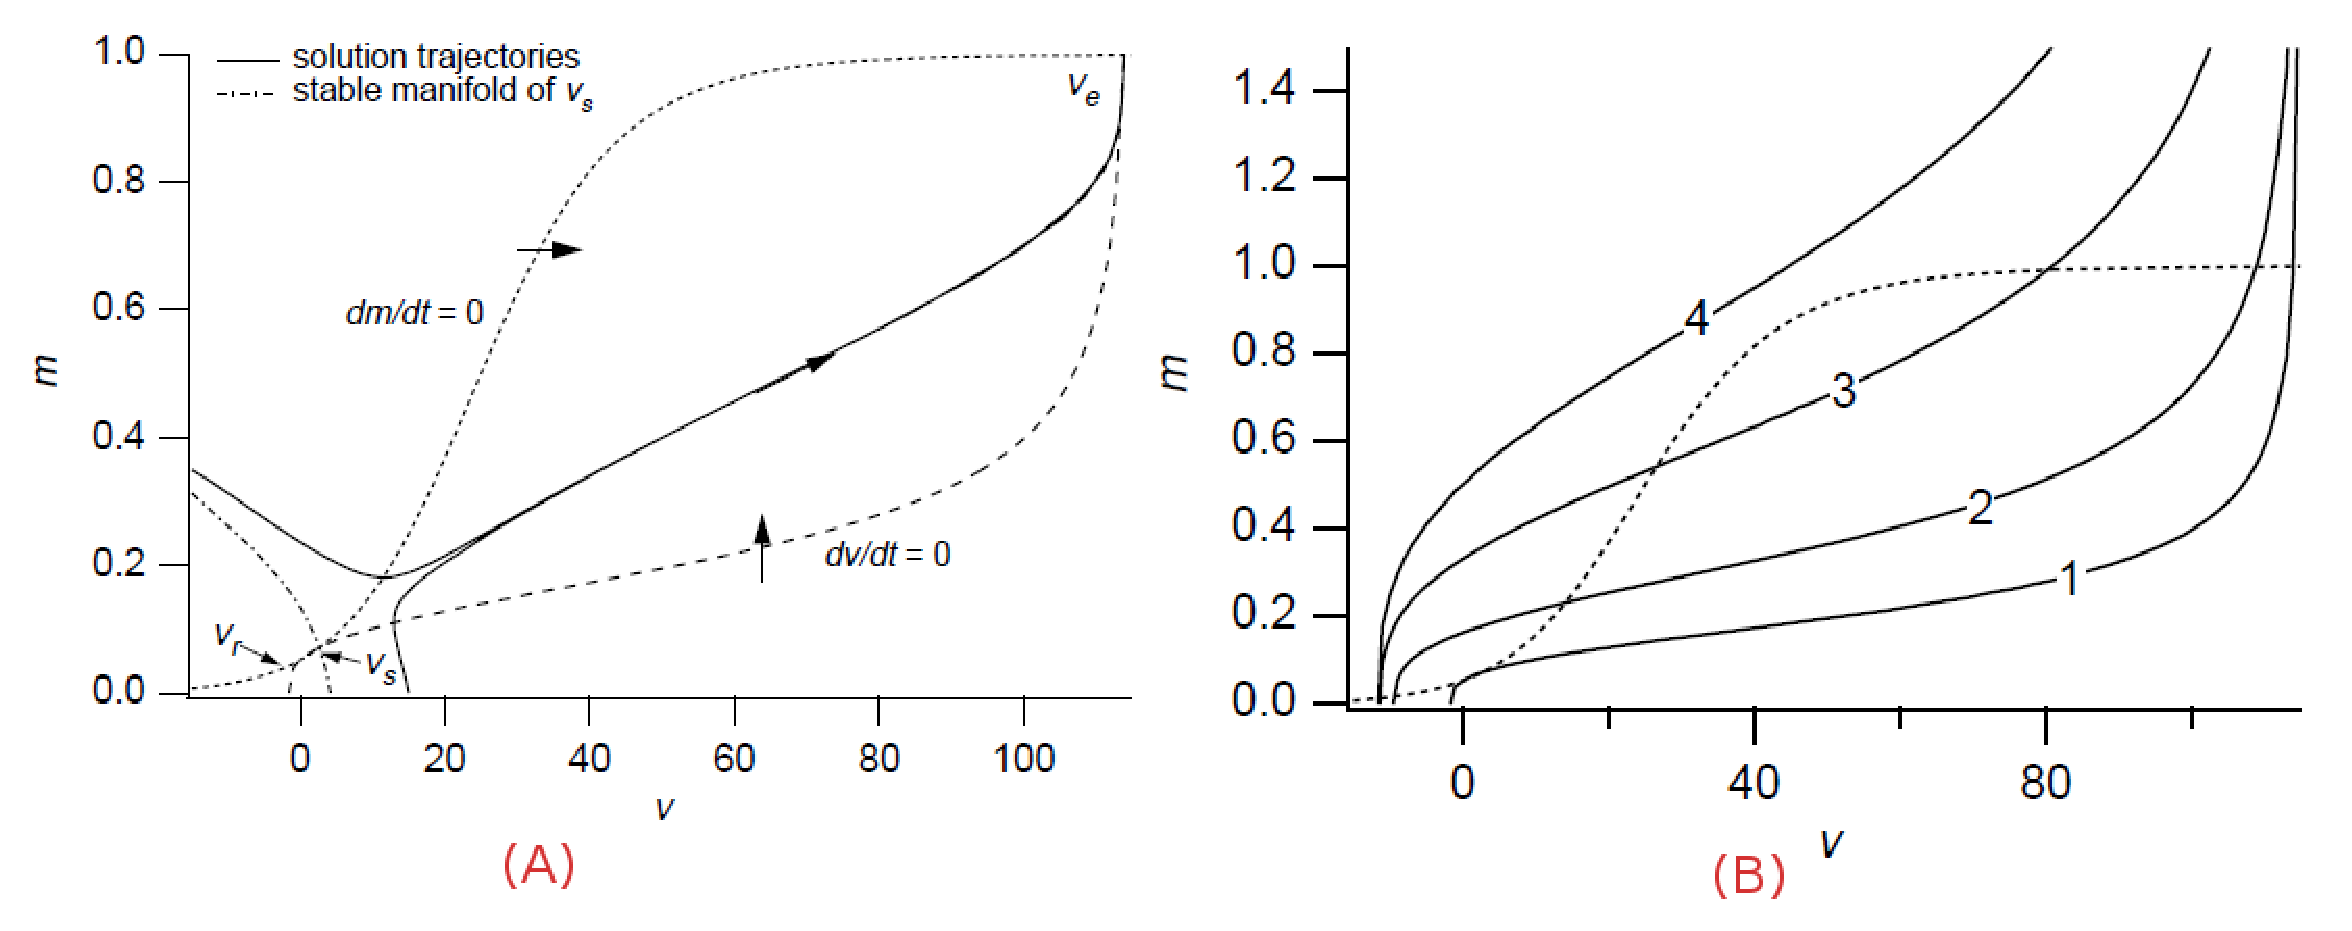
\includegraphics[height=5cm,
    angle=0]{./images/FN_nullcline.eps}}
  \caption{m-nullcline, v-nullcline~\citep{keener1998mp} (pg132) [{\it NOTE:
  Using the current membrane potential concept, the membrane potential values
  become  positive rather than negative as shown in the H-H original paper}],
  $v_r$ resting point, $v_s$ saddle point, $v_e$ excited point:  
  (A) use $n_0=0.3176, h_0=0.596$. The short/long dotted lines show the
  nullclines; while the two solid lines show two trajectories (phase curve) of
  the system at two diffeent initial choice of $(v(0),m(0))$.   (B)
  $v$-nullcline at different values of $n,h$: (1) $n_0=0.3176,
    h_0=0.596$, (2) $h_0=0.4, n_0=0.5$, (3) $h_0=0.2, n_0=0.7$, and (4)
    $h_0=0.1, n_0=0.8$. }
\label{fig:FN_nullcline}
\end{figure}

Here, the behavior of the $(v,m$) reduced system - {\bf fast phase-plane} is
shown Fig.~\ref{fig:FN_nullcline}. The choices of $h,n$ doesn't affect
$m$-nullclines, but affect v-nullclines. Depending the resting value of $(h,n)$,
$m$-nullclines and $v$-nullclines can intersect at 1, 2 or 3 different
locations. The three intersection are called singular points: $v_r$, $v_s$, and
$v_e$. They are the {\it stable resting point}, {\it threshold saddle point}
(i.e. any trajectory below this return to the resting state, above this reach
the excited point before returning to the resting via refractory process), and
{\it stable excited point}, as shown in Fig.~\ref{fig:FN_nullcline}(A) with
$h=0.596, n=0.317$. 

Here, the different choices of $(h,n)$ can give different expected outputs, in
terms of number of critical points of the system.
In the case of (4), there is no excited point at all, or the cell can never be
excited no matter how we trigger it.
This cause $v_e, v_r$ move also in the direction that decrease $v_e$. If
$v$-nullcline keeps moving left, while $m$ nullcline doesn't move, e.g. (4)
nullcline doesn't intersect with $m$ nullcline anymore, which means the excited
point and saddle point disappear, yielding $v_r$ the only steady state. Thus,
the system must return to the resting values. This, mathematically, explains the
{\it refractoriness of the system}, i.e. the period in which the cell cannot be
excited.


If we look at it closer, as shown in Fig.3 of the original paper, there's a line
called {\bf threshold separatrices} (or stable separatrices). Any initial
conditions of $(v(0),m(0))$ below this path, the reduced system will eventually
reach $v_r$; and if the initial conditions fall into the opposite side of this
path, the reduced system will eventually reach $v_e$. The saddle point is 1D
stable manifold. Clearly, any perturbation not across the stable manifold return
to the resting state, while if it pass the stable manifold, it reaches the
excited point. If there is a saddle point in the system, it behaves as an
all-or-none behavior. \textcolor{red}{Mathematically, when the saddle point is
disappeared, the graded behavior occurs.}


% Even though $m$-nullcline is independent of $n,h$, the $V$-nullclines is not, as
% shown in Fig.~\ref{fig:FN_nullcline}(B), it moves left and up. 


\begin{mdframed}

However, the two points $V_r,V_e$ in fact are pseudo-stable states of the
complete system. They are stable in the context of fast subsystem (i.e. $V_m$
stay at $V_e$ forever after it reaches this value), yet unstable in the complete
system.
\end{mdframed}

Next, the effect of the reduced system is analyzed by setting $h,n$ to a
different constant values or by changing $I_\app$ is investigated. Finally, $h$
and $n$ are introduced to the system separatedly, and then we study the new
reduced system ($(V,m,h)$ or $(V,m,n)$). This can give a better understanding of
the complete system, rather than considering all the variables at onces. From
this, they obtained one important understanding, i.e. which variables to change
to give the plateau-shaped AP, resembling those obtained experimentally in
muscle, cardiac cells, and even squid axon.

\begin{figure}[hbt]
  \centerline{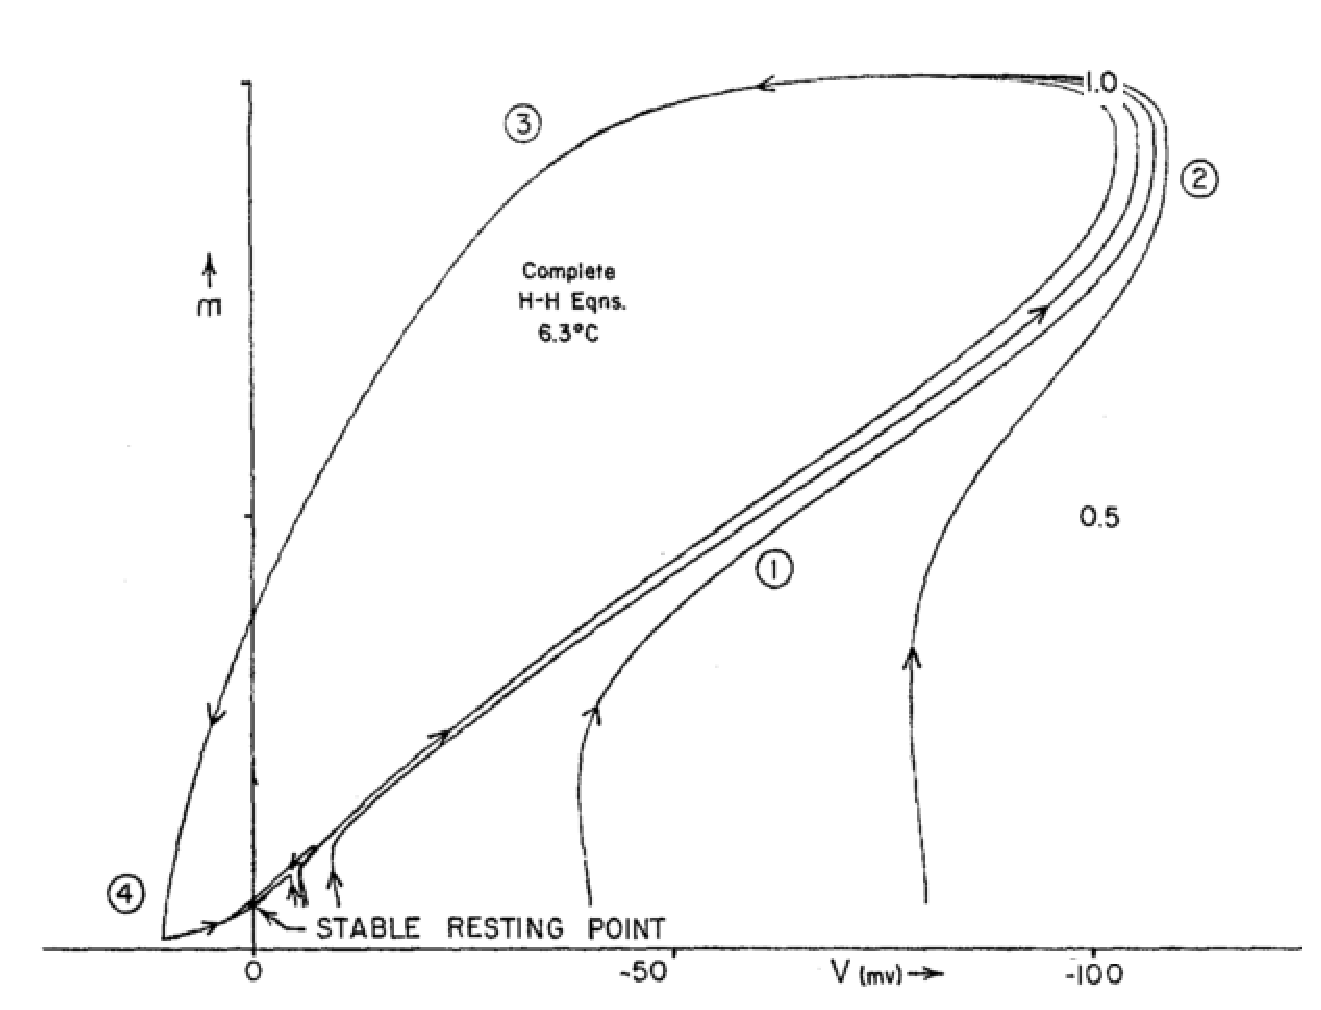
\includegraphics[height=5cm,
    angle=0]{./images/FitzHughFig9_phaseplane.eps}}
  \caption{(V,m) phase plane showing paths. Circle numbers shown the different
  phase of the AP corresponding to Fig.\ref{fig:FitzHugh1960_Vm}.}
  \label{fig:FN_phaseplane}
\end{figure}

An example of phase plane plot is shown in Fig.\ref{fig:FN_phaseplane}. In the
case of complete system, when it reaches $V_e$, $h_\infty(V_e)<h_\infty(V_r)$,
$n_\infty(V_e)>n_\infty (V_r)$. It means that the probability for NOT binding of
blocking molecule decreases. The powerful of phase-plane analysis is shown in
Fig.\ref{fig:FN_phaseplane2}.


\begin{figure}[hbt]
  \centerline{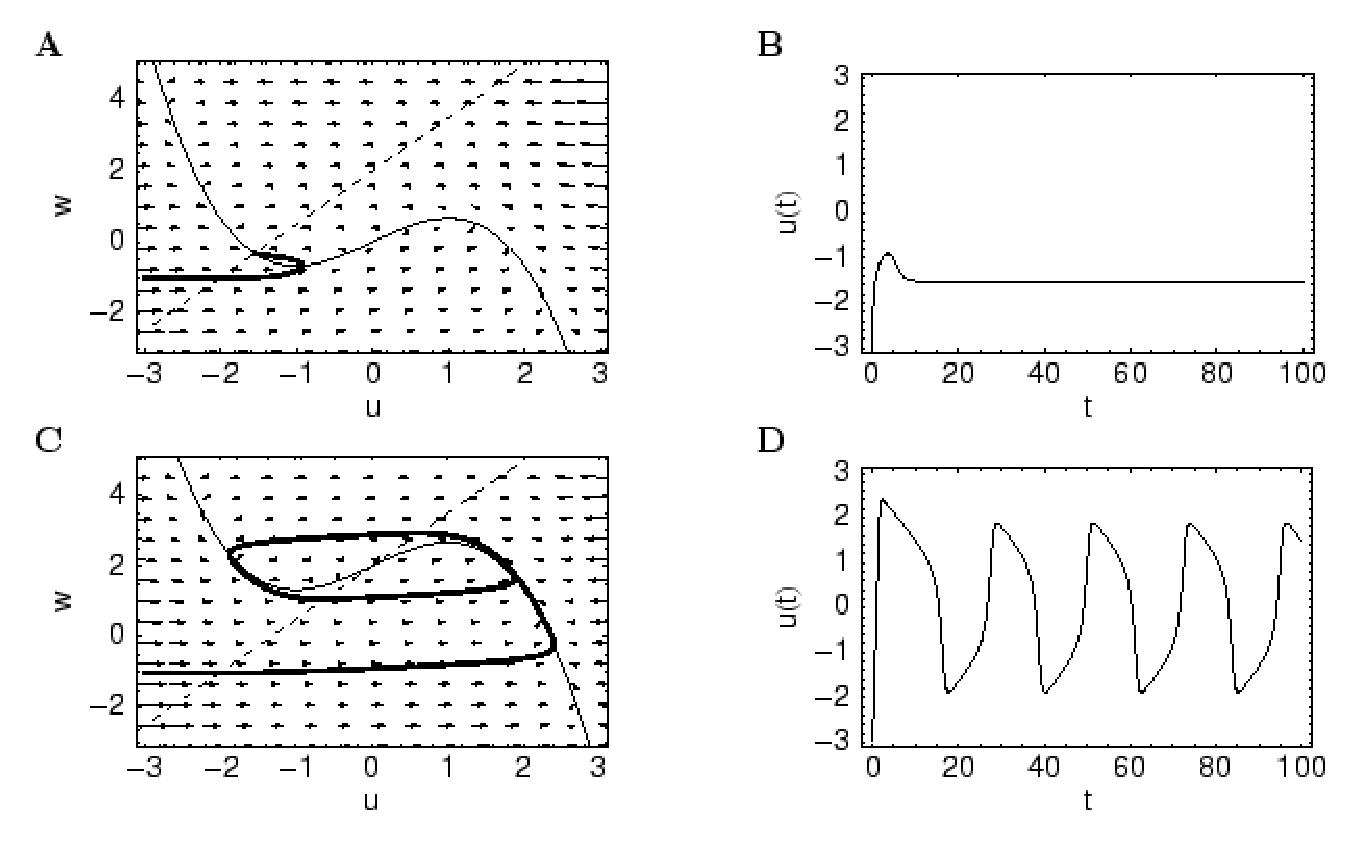
\includegraphics[height=5cm,
    angle=0]{./images/FitzHugh-phaseplane.eps}}
  \caption{Phase plane can help us tell how the system behave. (A) the system
  reaches the resting fixed-point and no oscillation as shown in (B). (C) the
  system reach a limit cycle, and infinite oscillation as shown in (D)}
  \label{fig:FN_phaseplane2}
\end{figure}

% \subsubsection{fast-slow phase-plane}
% \label{sec:fast-slow-phase}
\subsection{Fast-slow analysis}

In the previous
section, we investigate both fast kinetic variables $V_m$, and $m$. An
equivalent to BVP model is by taking a cross-section, i.e. investigate one fast
and one slow variable, it can provide another view into the system. They
observed that $n+h \approx 0.8$ (actually, it is 0.9), so $V$ and $n$ are examined in the
reduced system. $m$ is approximated as an instantaneous function of membrane
potential $m=m_\infty(V_m)$, and $h=0.8-n$.

\begin{equation}
  \label{eq:287}
  \begin{split}
    \Csc dV_m /dt =& - \overline{g_{\ce{K}}}.n^4(V_m -E_{\ce{K}}) - \overline{g_{\ce{Na}}}.
    m_\infty^3(V_m).(0.8-n).(V_m -E_{\ce{Na}}) - \\
    & \overline{g_{\leak}}.(V_m -E_{leak}) + I_\app\\
    \frac{dn}{dt} =& -\frac{n-n_\infty(V_m)}{\tau_n(V_m)}
  \end{split}
\end{equation}
NOTE: $m_\infty, n_\infty, \tau_n$ are instantaneous functions of $V_m$. So, we
can obmit them from the formula. A better arrangement for eq.~\eqref{eq:287} is
\begin{equation}
  \label{eq:604}
  \begin{split}
    \Csc dV_m /dt =& - \overline{g_{\ce{K}}}n^4(V_m -E_{\ce{K}}) -
     \overline{g_{\ce{Na}}} m_\infty^3(0.8-n)(V_m -E_{\ce{Na}}) - \\
	&     \overline{g_{\leak}} (V_m -E_{leak}) + I_\app\\
    \frac{dn}{dt} =& -(\alpha_n+\beta_n)n +\alpha_n
  \end{split}
\end{equation}


\begin{figure}[hbt]
  \centerline{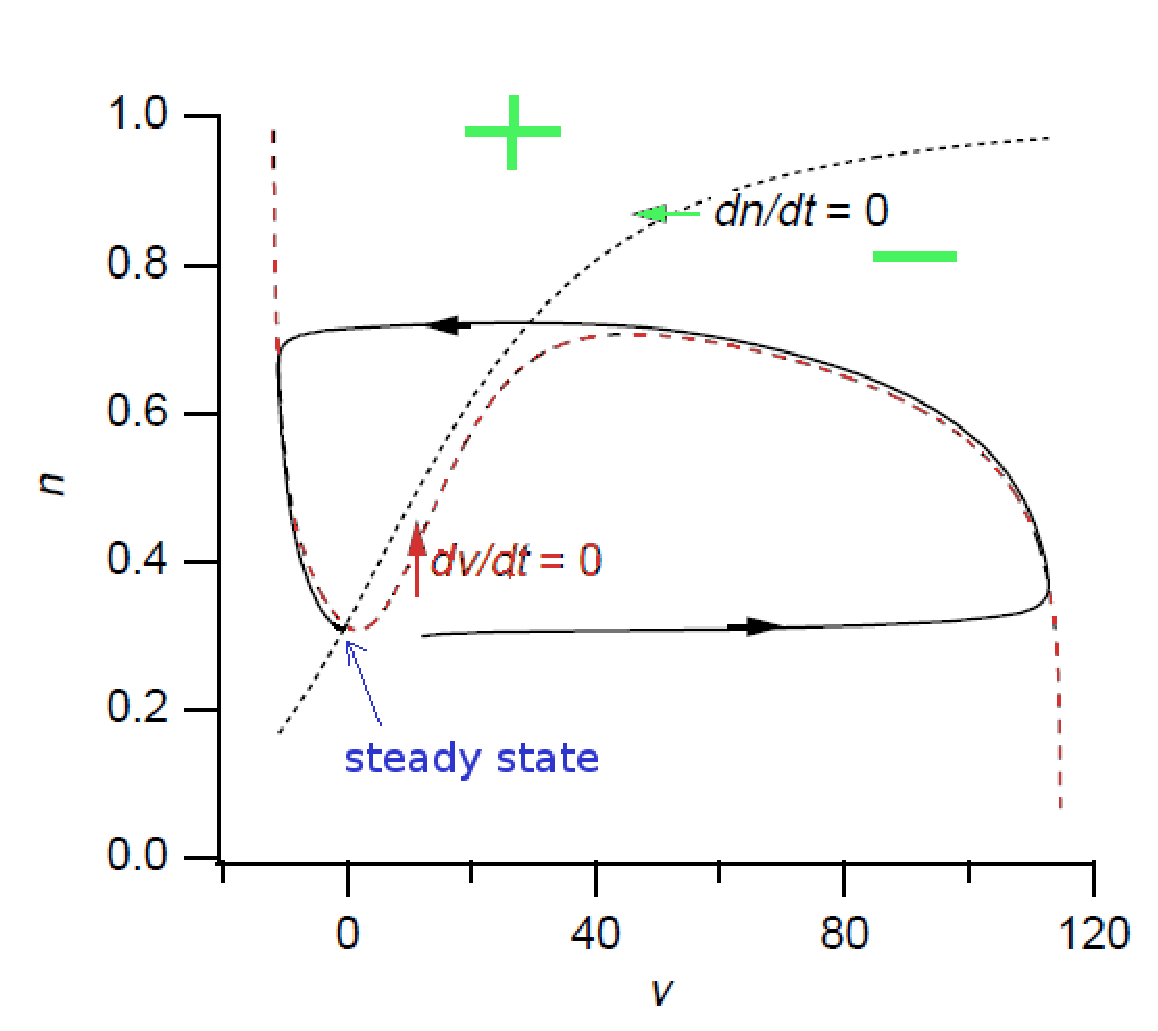
\includegraphics[height=5cm,
    angle=0]{./images/FN_fast_slow.eps}}
  \caption{Fast-slow phase-plane $(V_m,n)$}
  \label{fig:FN_fast_slow}
\end{figure}

This system has 2 dependent variables (V,n), $V$ is called the excitation
variable, and $n$ is recovery variable as $n$ pull the system returning to the
steady state. Without $n$, the solution would stay at the excited state
indefinitely. The nullclines are shown in Fig.\ref{fig:FN_fast_slow}. The
$n$-nullcline is $\frac{\alpha_n}{\alpha_n+\beta_n}$ which is the $n_\infty$,
black dotted line, and can be approximated by a straight line (within the
physiological range of the variables).
The $V$-nullcline, however, has a cubic shape, the red dotted line in
Fig.~\ref{fig:FN_fast_slow}.
Due to the fast kinetic of $V$ compared to $n$, the trajectory is almost
horizontal except at the point near $dv/dt\approx 0$.
That's why the curve $dv/dt=0$ is called the ``slow manifold'' as close to this
line, the solution move slowly in the direction determined by $dn/dt$.


% \begin{figure}[hbt]
%   \centerline{
\includegraphics[height=6cm,
%     angle=0]{./images/HH_reduced.eps}}
%   \caption{The trajectory of the AP in two reduced systems $(V,m)$,
%     (n,h) are projected into two lines $u=V_m+36m$, and $w=(n-h)/2$,
%     respectively. }
%   \label{fig:HH_reduced}
% \end{figure}
  


\subsection{Hopf bifurcation analysis}

%http://icwww.epfl.ch/~gerstner/SPNM/node22.html#SECTION02221000000000000000

The dimensionless form of FitzHugh-Nagumo model is
\begin{equation}
\label{eq:FH-N}
\begin{split}
\frac{dx}{dt} &= x(x-\alpha)(1-x) - y + I_\app \\
\frac{dy}{dt} &= \varepsilon (x-\gamma y)
\end{split}
\end{equation}
Some chose to use the form
\begin{equation}
\begin{split}
\frac{dx}{dt} &= \frac{1}{\varepsilon}(x(x-\alpha)(1-x) - y + I_\app) \\
\frac{dy}{dt} &= x-\gamma y
\end{split}
\end{equation}
with $x$ represents the fast variable (potential), and $y$ represents the slow
variable. $\alpha, \gamma, \varepsilon$ are constants with $0<\alpha<1$, and
$\varepsilon \ll 1$ (accounting for the slow inactivation kinetics of the
sodium channel); $\gamma > 0$ and small enough \citep{rinzel1990prop}. To obtain
supra-threshold behavior, ususally $\alpha< 0.5$ is chosen \citep{tuckwel2003}.

The variation of the parameters $\alpha, \gamma, \varepsilon$ can be associated
with some internal physiological change in the cell itself.  Here, $\alpha$
control the threshold between electrical silence and neuronal firing. $\alpha$
can also control the firing frequency and amplitude. \citep{faghih2010}
suggested that adding an additinal ODE of $\alpha$ to the system can give
bursting behavior.
\begin{equation}
\frac{d\alpha}{dt}=g(t)
\end{equation}
He successfully shown that tonic bursting, mixed mode firing, neural firing with
non-increasing frequency and varying frequency neural firing can be obtained
(using Simulink for simulation).  

The nullclines define $\dot{v}=0, \dot{w}=0$
\begin{eqnarray}
w &&= v - \frac{1}{3}v^3 + I_\app	\\
w &&= \frac{1}{b}(v+a) 
\end{eqnarray}
The intersection of nullclines are the fixed-points. Other parameters were 
chosen, when $I_\app$ increases, the system changes from a stable fixed-point to
a limit cycle (unstable fixed-point). The point where the transition occur is
called a {\bf bifurcation point}, which implies the real part of at least one
of the eigenvectors changes from negative to positive.
Here, $I_\app$ is the bifurcation parameter.
Eigenvalues method is often used to analyze the stability of the fixed-point
(Sect.\ref{sec:eigenvalues-method}). The stability loss in combination with an
emerging oscillation is called {\bf Hopf bifurcation}. If the oscillatory
solution, which appears at the Hopf bifurcation, is itself unstable, the
scenario is called {\bf subcritical Hopf bifurcation}. In the case of FH-N
model, the dynamics blows up and approach another limit cycle of larger
amplitude.


QUESTIONS: Using the dimensionless form, sketch two nullclines with $I_\app=0$,
and find the unique steady-state. When applying $I_\app\ne 0$, how it affects
the nullclines and the stability of the system? This can be done using {\bf
Hopf bifurcation analysis} with $I_\app$ as the bifurcation parameter. 

The system shows a bistability property which is predicted by theory and verfied
experimentally. A possible benefit of bistability is that the system can go on
continuous firing with only a transient, not necessarily steady, stimulus. 

It's a common practice to represent a dynamical system using its bifurcation
diagram. \citep{kostova2004} pointed out that the possible number of 
bifurcation diagrams for the FitzHugh-Nagumo model is 8,
Fig.\ref{fig:FitzHugh-bifurcation}.
\begin{enumerate}
  \item saddle-node bifurcations of equilibria and subcritical Hopf bifurcations
  \item saddle-node bifurcation of periodic orbits and homoclinic bifurcations
  (which occur in a very narrow interval of magnitude $10^{-7}$ values of
  $I_\app$).
\end{enumerate}

\begin{figure}[hbt]
  \centerline{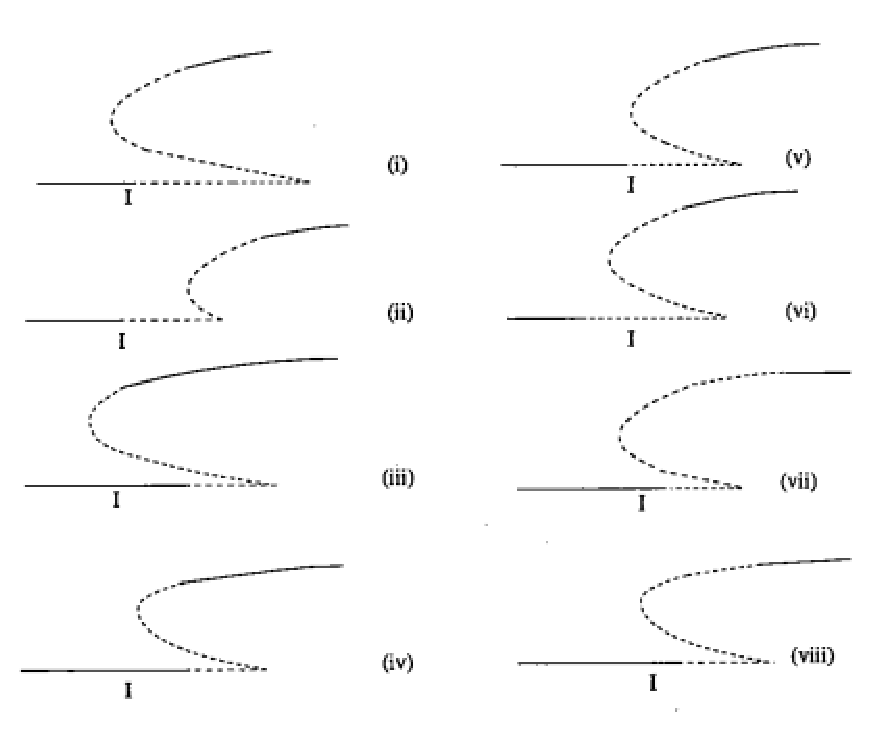
\includegraphics[height=5cm,
    angle=0]{./images/FitzHugh-8-bifurcations.eps}}
  \caption{Eight possible bifurcation curves}
  \label{fig:FitzHugh-bifurcation}
\end{figure}

Each bifurcation phenomena is the result of modifying one parameter. Consider
eq.\eqref{eq:FH-N}. Let $(v_{eq}, w_{eq})$ be the equilibrium point, and define
$f(v)=v(v-\alpha)(1-v)$. Then, the equation can be rewriten in the form
\begin{eqnarray}
\frac{dv}{dt} = f(v+v_{eq})-f(v_{eq}) - w \\
\frac{dw}{dt} = \varepsilon (v- \gamma w)
\end{eqnarray}
The mathemtical background behind bifurcation is complicated, yet we can use
some existing tools to generate the bifurcation (e.g. XPPAUT)
(Sect.\ref{chap:bifurcation-theory}). 

QUESTION: Given $\varepsilon=0.1, \beta=0.5$, check what values of $\alpha$ so
the system undergoes a Hopf bifurcation. Then, use XPPAUT to plot the
bifurcation diagram for this system
 \footnote{\url{http://slesse.math.ubc.ca/wikis/Courses/index.php/Math_361/Problems/A_Hopf_bifurcation_in_the_FitzHugh-Nagumo_system}}.



\subsection{Data analysis}

\citep{tasaki1957}
showed that using tetraethylammonium chlorine (TEA) in squid nerve can reproduce
the long AP. Computationally, this can be reproduce by multiplying the time
constant of $n$ by 100 or more, and that of $h$ by 1/3 \citep{fitzhugh1960tph}.
The plateau range in AP is similar to what observed in muscle cells,
Fig.\ref{fig:FN_plateauVm}. However, the theoretical membrane conductance curves
differ significantly from experimental ones.

\begin{figure}[htb]
  \centerline{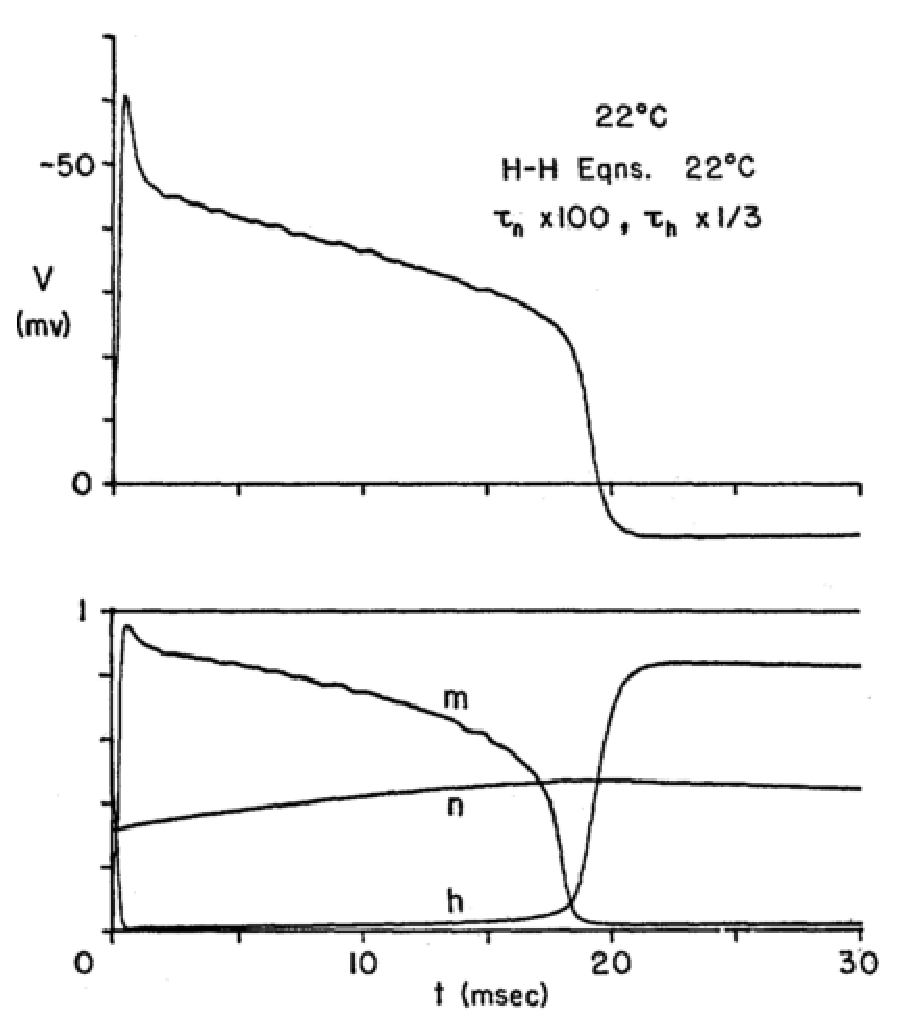
\includegraphics[height=5cm]{./images/FitzHugh1960_plateauVm.eps}}
  \caption{Modified the time constants of $h,n$ give a prolonged AP with a
  finite plateau. The models run at 22$^\circ$C, after adjusing the parameter
  using Q10 as described in Sect.\ref{sec:q10-factor}}
  \label{fig:FN_plateauVm}
\end{figure}
 
In Hodgkin-Huxley model, a constant current steps can produce finite/infinite
trains of impulses (i.e. damped or undamped), Fig.12 (in the paper). The
infinite trains of impulses appear in the phase space as {\it stable limit
cycles}. In BVP model, the limit cycle appears when the singular point (the
resting point P) becomes unstable. Experimentally, in excised squid giant axons,
only short finite trains occur. This presents a major disagreement between HH
model and the real axon. To avoid infinite trains of impulses,
\citep{fitzhugh1961ips} suggested that an augmented term to be added to the
equation, to make the singular point from unstable to stable. 

A year later, \citep{fitzhugh1961ips} produced a BVP model. However, the model
doesn't intend to be an accurate quantitative model of the axon (in the sense
of reproducing the shape of experimental curves). Nevertheless, it exhibits
basic dynamic relationship between variables of states: properties of threshold,
refractoriness, finite and infinite trains of impulses. Then, an equivalent
to BVP model using Hodgkin-Huxley model was introduced that can reproduce {\bf
tonic firing}, i.e. a firing behavior in which the neuron spikes in a periodic
manner, Fig.\ref{fig:tonic_firing}. However, the model cannot reproduce certain
behaviors, such as bursting. Bursting behavior can be reproduced in
Hindmarsh-Rush model.
 

\begin{figure}[htb]
  \centerline{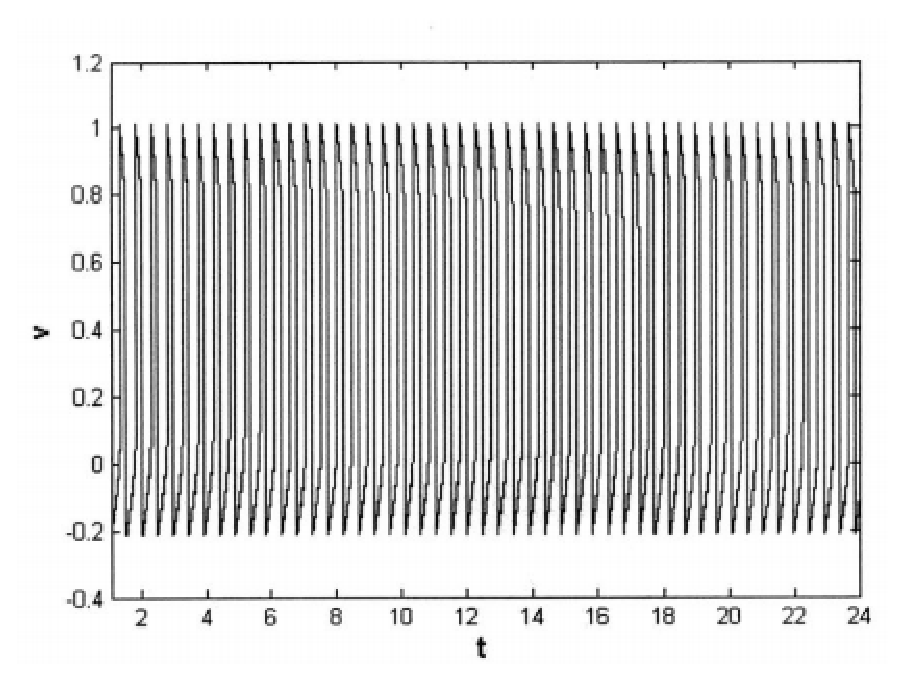
\includegraphics[height=5cm]{./images/tonic_firing.eps}}
  \caption{Tonic firing}
  \label{fig:tonic_firing}
\end{figure}
 
 Both BVP model and Hodgkin-Huxley model contain a quasi-threshold phenomemon,
 i.e. excitability is an all-or-none process. Graded
 responses of membranes which is important in neural integration cannot be
 reproduced by the models.
 
 Further studies of the models include \cite{kostova2004, faghih2010}.
 
\section{Other cell models}

\begin{enumerate}
 \item dimension-less oscillation: Sect.\ref{sec:Hindmarsh-Rush_model}
 
 \item low-threshold spiking: only need T-type $\Ca$ channel
 - Sect.\ref{sec:Wang-1991-thalamic-relay-neuron}
 
 \item A-type mediated LTS : Sect.\ref{sec:McCormick-Huguenard-1992}
 
 \item LTS-mediated bursting: need T-type $\Ca$ channel and two components for
 generating AP ($\Na$ and delayed-rectified $\K$ current) -
 Sect.\ref{sec:Rush-Rinzel-1994}

 \item Refine burst and spike patterns: 
 need L-type calcium current, a calcium-activated potassium current (SK or BK),
 a persistent sodium current (Nap), a transient potassium current (IA), and a
 hyperpolarization-activated 'sag current', Ih (Sect.\ref{sec:HCN-channels})
  
NOTE: HCN carries Na+ and K+ ions and has a reversal potential of around -40mV.
It contributes to the slow depolarization between bursts and helps to set the
slower rhythm (0.5-4 Hz) seen with increased hyperpolarization during deeper
sleep states.
  
 Example: (Lytton and Sejnowski 1992; McCormick and Huguenard 1992;
Rose and Hindmarsh 1989c) 

  \item generate spindling rhythm: (Destexhe et al. 1994). - Sect.\ref{sec:Destexhe-Mainen-Sejnowski-1994}

  \item simultaneous effects of T-type $\Ca$ channel and Ih: Wang 1994; Wang and
  Rinzel 1995?
  
  \item More advanced models: that include cable properties of (thalamic)
  neurons
\end{enumerate}


 

